\documentclass[12pt]{article}
\usepackage{graphicx} % Required for inserting images
\usepackage[utf8]{inputenc}
\usepackage[T2A]{fontenc}
\usepackage[russian]{babel}
\usepackage{amsfonts}
\usepackage{amsmath}
\usepackage{amssymb}
\usepackage{fancyhdr}
\usepackage{float}
\usepackage[left=2cm,right=2cm,top=2.5cm,bottom=2.5cm]{geometry}
\usepackage{graphicx}
\usepackage{hyperref}
\usepackage{indentfirst}
\usepackage{multicol}
\usepackage{stackrel}
\usepackage{xcolor}
\usepackage{yhmath}
\usepackage{stmaryrd}
\usepackage{enumitem}
\usepackage{fancyvrb}
\usepackage{listings}
\date{December 2024}
\begin{document}

\begin{quote}

\begin{center}
    \large Отчёт по лабораторной работе №5
\end{center}

\begin{center}
    \large Управление памятью в ОС Linux
\end{center}

\begin{center}
    \normalsize Жунусов Данияр M3233
\end{center}

Данные о текущей конфигурации операционной системы
\begin{itemize}
  \item Общий объем оперативной памяти: 4010504 kB
  \item Объём раздела подкачки: 2744316 kB
  \item Размер страницы виртуальной памяти: 4 kB
  \item Объем свободной физической памяти в ненагруженной системе: 1367908 kB
  \item Объем свободного пространства в разделе подкачки в ненагруженной системе: 2744316 kB
\end{itemize}

\begin{center}
    \normalsize Эксперимент №1 
\end{center}

\begin{center}
    \normalsize Первый этап
\end{center}

\begin{center}
    \normalsize Запущенный скрипт
\end{center}

\begin{figure}[h]
    \centering
    \includegraphics[width=0.7\textwidth]{script.png}
    \caption{mem.bash}
    \label{fig:example}
\end{figure}

Наблюдение после запуска скрипта

\begin{figure}[h]
    \centering
    \includegraphics[width=1\textwidth]{top.jpg}
    \caption{Запущенный скрипт появился в top}
    \label{fig:example}
\end{figure}

\begin{figure}[h]
    \centering
    \includegraphics[width=1\textwidth]{top 2.jpg}
    \caption{Спустя 20 секунд скрипт занял около 2,3 Гб физической памяти}
    \label{fig:example}
\end{figure}

\begin{figure}[h]
    \centering
    \includegraphics[width=1\textwidth]{top 3.jpg}
    \caption{Спустя 1 минуту скрипт занял всю доступную физическую память и начался процесс подкачки (swap)}
    \label{fig:example}
\end{figure}

\begin{figure}[h]
    \centering
    \includegraphics[width=1\textwidth]{top 4.jpg}
    \caption{Спустя 1.5 минуты скрипт всю свободную память после чего аварийно завершился}
    \label{fig:example}
\end{figure}


\clearpage

\lstset{ 
  breaklines=true, 
  basicstyle=\ttfamily, 
  columns=flexible, 
  extendedchars=true
}

Последние две записи о скрипте в системном журнале: 
\begin{lstlisting}
[  192.131240] oom-kill:constraint=CONSTRAINT_NONE,nodemask=(null),cpuset=/,mems_allowed=0,global_oom,task_memcg=/user.slice/user-1000.slice/user@1000.service/app.slice/app-org.gnome.Terminal.slice/vte-spawn-83e765f0-27da-46d5-a532-06d4429f1941.scope,task=mem.bash,pid=2247,uid=1000

[  192.131262] Out of memory: Killed process 2247 (mem.bash) total-vm:5835536kB, anon-rss:3515776kB, file-rss:0kB, shmem-rss:0kB, UID:1000 pgtables:11460kB oom_score_adj:0
\end{lstlisting}

Значение в последней строке файла report.log: 74'000'000

\begin{figure}[h]
    \centering
    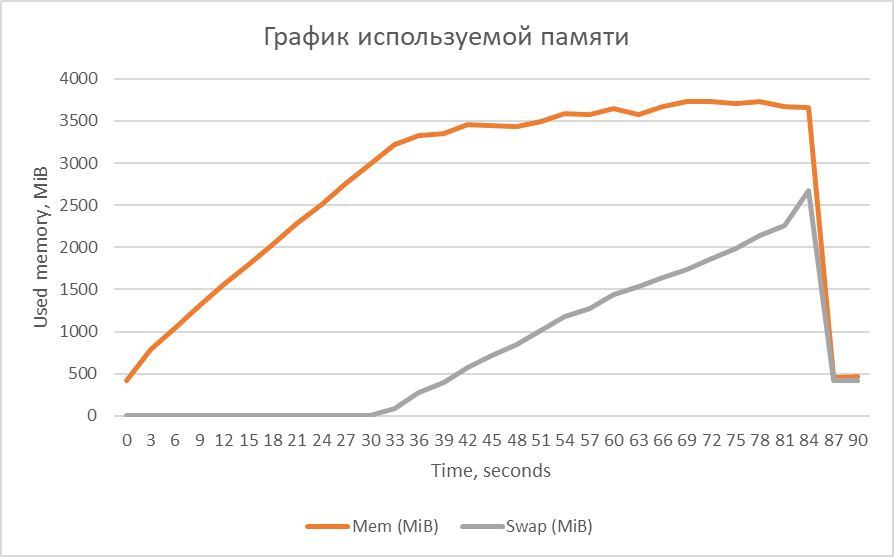
\includegraphics[width=0.7\textwidth]{image.png}
    \label{fig:example}
\end{figure}

На графике видно, что использование физической памяти перестало увеличиваться одновременно с началом заполнения раздела подкачки. Это произошло из-за исчерпания доступной физической памяти, после чего система начала использовать swap для хранения неактивных данных. Рост обеих метрик прекратился, когда физическая память достигла своего предела в 3.7 Гб, а раздел подкачки — 2.7 Гб. По завершении заполнения памяти система аварийно завершила работу скрипта, так как свободной памяти больше не осталось.

\begin{center}
    \normalsize Второй этап
\end{center}

\begin{center}
    \normalsize Запущенный скрипт
\end{center}

\begin{figure}[h]
    \centering
    \includegraphics[width=0.2\textwidth]{start12.png}
    \caption{run12.bash}
    \label{fig:example}
\end{figure}

\begin{figure}[h]
    \centering
    \includegraphics[width=0.7\textwidth]{mem2.png}
    \caption{mem2.bash}
    \label{fig:example}
\end{figure}

\begin{figure}[h]
    \centering
    \includegraphics[width=1\textwidth]{top12.png}
    \caption{После запуска run12.bash оба скрипта появились в top}
    \label{fig:example}
\end{figure}

\begin{figure}[h]
    \centering
    \includegraphics[width=1\textwidth]{top121.png}
    \caption{Спустя 20 секунд каждый скрипт занял по 1.5 Гб физической памяти}
    \label{fig:example}
\end{figure}

\begin{figure}[h]
    \centering
    \includegraphics[width=1\textwidth]{top122.jpg}
    \caption{Спустя 35 секунд скрипты заняли всю память после чего mem.bash был аварийно остановлен}
    \label{fig:example}
\end{figure}

\begin{figure}[h]
    \centering
    \includegraphics[width=1\textwidth]{top123.jpg}
    \caption{Из-за аварийной остановки скрипта mem.bash память, выделенная ему, была освобождена. После этого освобожденная память стала доступна другим процессам, включая запущенный параллельно скрипт mem2.bash, который занял её для выполнения своих операций.}
    \label{fig:example}
\end{figure}

\begin{figure}[h]
    \centering
    \includegraphics[width=1\textwidth]{top124.jpg}
    \caption{Спустя 1 минуту скрипт mem2.bash занял всю память, после чего был аварийно остановлен.}
    \label{fig:example}
\end{figure}

\clearpage

Последние записи в системном журнале:
\begin{lstlisting}
[ 1230.694152] oom-kill:constraint=CONSTRAINT_NONE,nodemask=(null),cpuset=/,mems_allowed=0,global_oom,task_memcg=/user.slice/user-1000.slice/user@1000.service/app.slice/app-org.gnome.Terminal.slice/vte-spawn-19c30427-8b18-46e7-8dba-ab7787912078.scope,task=mem.bash,pid=2456,uid=1000
[ 1230.694168] Out of memory: Killed process 2456 (mem.bash) total-vm:2925860kB, anon-rss:1797120kB, file-rss:0kB, shmem-rss:0kB, UID:1000 pgtables:5768kB oom_score_adj:0
[ 1268.604826] [   2457]  1000  2457  1457861   880320   880320        0         0 11726848   575040             0 mem2.bash
[ 1268.604831] oom-kill:constraint=CONSTRAINT_NONE,nodemask=(null),cpuset=/,mems_allowed=0,global_oom,task_memcg=/user.slice/user-1000.slice/user@1000.service/app.slice/app-org.gnome.Terminal.slice/vte-spawn-19c30427-8b18-46e7-8dba-ab7787912078.scope,task=mem2.bash,pid=2457,uid=1000
[ 1268.604849] Out of memory: Killed process 2457 (mem2.bash) total-vm:5831444kB, anon-rss:3521280kB, file-rss:0kB, shmem-rss:0kB, UID:1000 pgtables:11452kB oom_score_adj:0
\end{lstlisting}

Значение в последней строке файла report.log: 37'000'000

Значение в последней строке файла report2.log: 74'000'000

\begin{figure}[h]
    \centering
    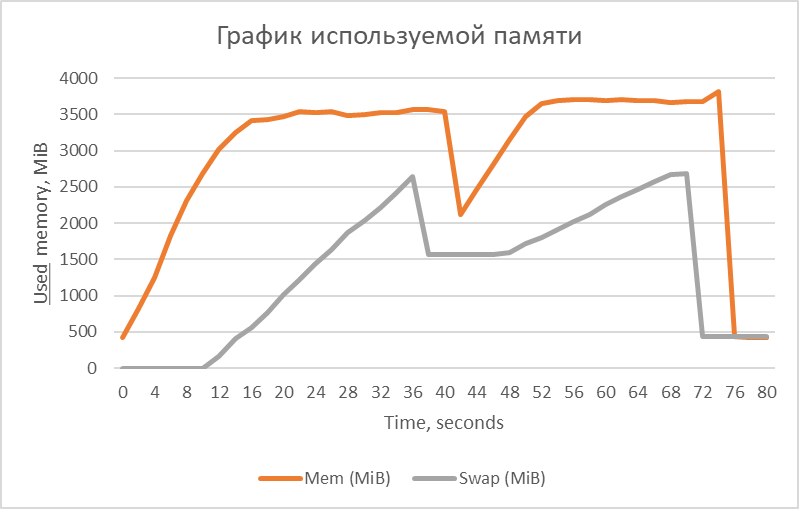
\includegraphics[width=1\textwidth]{graph2.png}
    \label{fig:example}
\end{figure}

\begin{figure}[h]
    \centering
    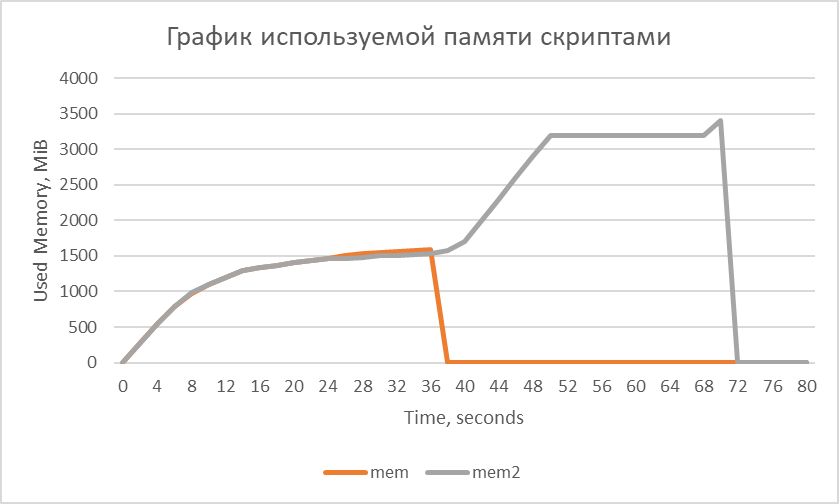
\includegraphics[width=1\textwidth]{graph3.png}
    \label{fig:example}
\end{figure}

\clearpage

Выводы: На первом этапе эксперимента работающий процесс постепенно заполнил всю доступную физическую память, что привело к активации механизма подкачки, после чего был заполнен и раздел подкачки. Как только ресурсы виртуальной памяти оказались исчерпаны, процесс завершился аварийно, поскольку система больше не могла выделить новые страницы ни в физической, ни в виртуальной памяти.
Во втором этапе процессы завершались поочередно: первым завершился mem.sh, так как на момент исчерпания памяти он использовал её больше, чем mem2.sh. После освобождения памяти первым процессом, mem2.sh продолжил выполнение, используя доступные ресурсы, однако позже также был завершён системой.

\clearpage

\begin{center}
    \normalsize Эксперимент №2
\end{center}

Сначала запускаем скрипт с параметрами $n = 7400000$ (размер массива в 10 раз меньший при котором происходила аварийная остановка) и $k = 10$. Все запуски успешно завершились и в системном журнале нет записей об аварийной остановке. Увеличиваем значение $k$ до 30. При этом некоторые процессы завершились аварийно из-за того, что закончилась свободная память.Используя скрипт find2.bash, который выполняет бинарный поиск, определяем максимальное значение $N$, при котором все процессы успешно завершаются.
В результате выясняем, что $N =$ 5875000.


Выводы: В ходе эксперимента был проведен анализ влияния размера массива ($N$) и количества запусков скрипта ($k$) на возможность аварийных завершений процессов. При значении $k =$ 10 все запуски скрипта завершились успешно, без аварийных остановок. При увеличении значения $k$ до 30 запусков, наблюдались аварийные завершения некоторых процессов. Далее было найдено максимальное значение N, которое позволяет избежать аварийных завершений процессов при $k =$ 30. Это значение составляет 5875000.

\end{quote}

\end{document}
